


    \section{Aufbau}

        
        \begin{figure}[H]
            \centering
            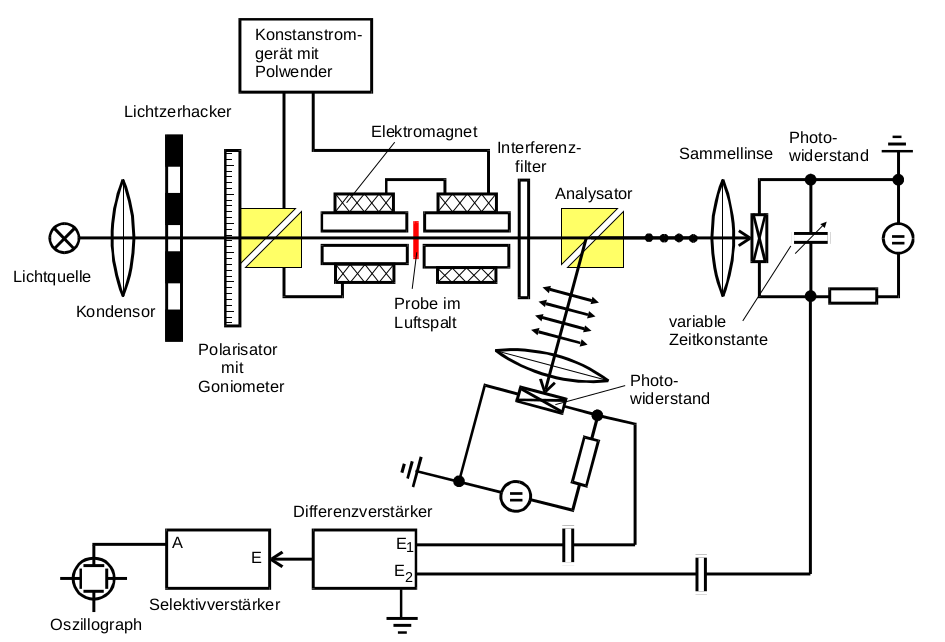
\includegraphics[height=5cm]{aufbau.png}
            \caption{Versuchsaufbau zum vermessen des Zeeman-Effekts an einer Cadmium-Lampe \cite{anneu}.}
            \label{fig:aufbau}
        \end{figure}

        Ein Bild des Aufbaus ist in Abb. \ref{fig:aufbau} zu sehen.
        Die verwendete Lichtquelle besteht aus Cadmium und sendet verschiedenfarbige 
        Linien aus, unter anderem rote und blaue. Sie befindet sich in einem Elektromagneten, 
        welcher so geöffnet ist, dass das transversal emittierte Licht von 
        optischen Elementen aufgefangen werden kann. 
        Das Licht passiert ein Okular und eine Sammellinse, bevor es auf einen dünnen 
        Spalt trifft. Danach wird es durch eine Linse wieder aufgefächert und durchtritt ein 
        Geradsichtprisma, welches das Licht in seine unterschiedlichen Wellenlängen aufspaltet. 
        Dem Prisma folgen ein drehbarer Polarisator, eine Sammellinse und ein weiterer Spalt, 
        mit dessen Hilfe eine einzige der zuvor separierten Farben ausgewählt werden kann. 
        Nach einer weiteren Sammellinse trifft das Licht auf das Prisma einer Lummer-Gehrcke-Platte (siehe Abb. \ref{fig:lummer}). 

        \begin{figure}
            \centering
            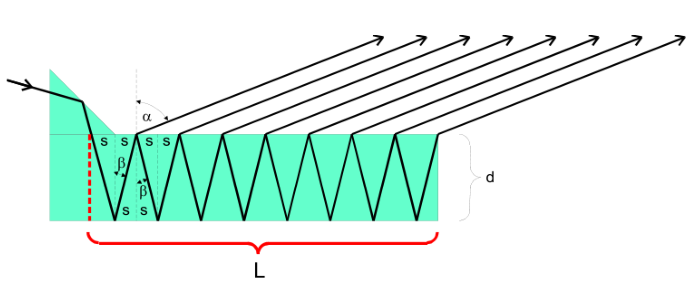
\includegraphics[height=5cm]{lummer.png}
            \caption{Strahlengang innerhalb einer Lummer-Gehrcke-Platte \cite{anneu}.}
            \label{fig:lummer}
        \end{figure}

        Die eigentliche Platte besteht aus zwei planparallelen Platten, zwischen welchen 
        das Licht größtenteils reflektiert wird. Interferenz entsteht dadurch, dass bei jeder 
        Reflexion auch ein kleiner Anteil des Lichts austritt. Diese Anteile interferieren für 

        \begin{equation}
            2\, n\, d\, \symup{cos}(\beta) = m\lambda,
        \end{equation}

        wobei $n$ und $d$ Brechungsindex und Dicke der Platte darstellen und $\beta$ der
        Einfallswinkel in die Platte ist. Nach der Platte trifft das Interferenzmuster auf eine 
        Kamera, durch die es festgehalten wird.



\section{Durchführung}
\label{sec:Durchführung}


        \subsection{Eichung des Magnetfeldes}

            In dieser Eichung soll der Zusammenhang zwischen dem angelegten Strom und 
            dem resultierenden Magnetfeld innerhalb der Polschuhe des Elektromagneten 
            gefunden werden. Dazu wird in drei Messdurchgängen 
            die Stromstärke im Bereich zwischen 1 und 19\,A in 1\,A-Schritten variiert
            und das zugehörige Magnetfeld mithilfe einer Hallsonde gemessen.

        \subsection{Justage der optischen Elemente}

            Zunächst wird das Licht durch Verschiebung der ersten Linse und des Objektivs 
            so verändert, dass es am ersten Spalt scharf ankommt. Danach wird durch Verschiebung 
            der zweiten Linse garantiert, dass das Lichtbündel parallel und nicht größer als 
            das Prisma auf das Geradsichtprisma trifft. Auf den zweiten Spalt muss das Licht 
            ebenfalls mit einer Sammellinse fokussiert werden. Um den Strahlengang in der 
            Lummer-Gehrcke-Platte erkennen zu können, wird die Linse horizontal so verschoben, 
            dass das grüne Licht vom Spalt durchgelassen wird, da dieses die höchste Intensität 
            besitzt. Eine Linse nach dem Spalt dient dazu, die ausgewählte Farbe in der richtigen 
            Größe auf das Eingangsprisma der Lummer-Gehrcke-Platte zu bringen. Der Winkel der Platte 
            muss im Folgenden so verändert werden, dass zwischen den planparallelen Platten Licht 
            hin- und herreflektiert wird. Zuletzt muss die Kamera so aufgestellt werden, dass 
            sie das Interferenzmuster der Platte aufnehmen kann.

        \subsection{Vermessung der roten Cadmium-Linie}

            Mithilfe einer Linse wird nur der rote Anteil des Lichts durch den Spalt 
            vor der Lummer-Gehrcke-Platte gelenkt. Zunächst wird mit der Digitalkamera 
            ein Bild des Interferenzmusters bei abgeschaltetem Magnetfeld aufgenommen. 
            Anschließend wird bei einem Strom von 10\,A ein Bild aufgenommen, auf dem
            der Übergang $\Delta m = 0$ nicht zu sehen ist, weil er durch den Polarisationsfilter 
            unterdrückt wird. Danach wird der Polarisationsfilter um 90° gedreht, um die Linie 
            dieses Übergangs ebenfalls sichtbar zu machen.

        \subsection{Vermessung der blauen Cadmium-Linie}

            Durch eine Linse und einen Spalt gelangt nur blaues Licht bis zur Lummer-Gehrcke-Platte. 
            Es muss darauf geachtet werden, dass die richtige der zwei blauen Linien untersucht wird. 
            Für diese wird zuerst eine Messung bei abgeschaltetem Magnetfeld durchgeführt. 
            Im Anschluss wird das Magnetfeld auf 6\,A eingestellt, damit die zwei $\sigma$-Linien 
            sichtbar gemacht werden können. Diese sind eventuell erst nach Drehung am Polarisationsfilter
            zu sehen. Nach einer Drehung des Polarisators um 90° und einer Felderhöhung auf 
            19\,A sind die zwei $\pi$-Linien mithilfe der Kamera zu erkennen.
